\documentclass{article}

\usepackage{amsmath, amsthm, amssymb, amsfonts}
\usepackage{graphicx}
\usepackage{setspace}
\usepackage{geometry}
\usepackage{float}
\usepackage{hyperref}
\usepackage[utf8]{inputenc}
\usepackage[english]{babel}

\newtheorem{theorem}{Theorem}[section]
\newtheorem{proposition}[theorem]{Proposition}
\newtheorem{principle}[theorem]{Principle}
\newtheorem*{remark}{Remark}

\setstretch{1.2}
\geometry{
    textheight=9in,
    textwidth=5.5in,
    top=1in,
    headheight=12pt,
    headsep=25pt,
    footskip=30pt
}

\begin{document}

\title{Information, Codes and Ciphers \\
       \vspace{.625em} Summary Notes \footnote{Based on MATH3411, UNSW 20T3.}}
\author{Hao Ren}
\date{November 2, 2020}
\maketitle

\newpage

\tableofcontents

\newpage

\setcounter{section}{-1}

\section{All TODOs}

Updated when \emph{3.X Compression Coding} finished as Version 1.

\subsection{Unfinished Contents}

\begin{itemize}
    \item 3.1.3 Decision Trees
    \item 3.2.4 Extensions of Huffman Coding
    \item 3.3.3 Huffman Coding for Stationary Markov Sources
    \item 3.4.2 Decoding: add a list to show steps like the one in 3.4.2 part.
    \item 3.6.x Other types of Compression
\end{itemize}

\subsection{Examples and Diagrams}

\begin{itemize}
    \item 3.2.3 Eg and Dia: Radix $r$ Huffman Codes
    \item 3.3.1 Eg: Definition of Markov Sources
    \item 3.3.3 Eg: with Huffman coding for Markov Sources
    \item 3.4.x Eg: Arithmetic encoding and decoding
    \item 3.5.x Eg: Dictionary Methods
\end{itemize}

\subsection{Proofs}

\begin{itemize}
    \item Theorem 3.1 The Kraft-McMillan Theorem
    \item Theorem 3.2 Minimal UD-codes
    \item Theorem 3.3 Huffman Code Theorem
    \item Proposition 3.4 Knuth
\end{itemize}

\newpage

\setcounter{section}{2}

\section{Compression Coding}

\subsection{Variable Length Encoding}

\begin{align*}
    \text{a source } S \qquad &\text{ with } q \text{ source symbols} \qquad & s_{1},s_{2},\cdots,s_{q},\\
    &\text{ with probabilities} \qquad &  p_{1},p_{2},\cdots,p_{q},\\
    \text{encoded by a code } C \qquad &\text{ with } q \text{ codewords} \qquad & c_{1},c_{2},\cdots,c_{q},\\
    &\text{ of lengths} \qquad & l_{1},l_{2},\cdots,l_{q}.
\end{align*}

\begin{itemize}
    \item with a radix $r$ codewords,
    \item variable length codes,
    \item not channel noise for source coding.
\end{itemize}

\subsubsection{UD and I-code}

A code $C$ is

\begin{description}
    \item[UD] uniquely decodable codes if it can always be decoded unambiguously,
    \item[I-code] instantaneous if no codeword is the prefix of others.
\end{description}

\subsubsection{Comma Codes}

The standard comma code of length $n$ is

\begin{itemize}
    \item a code which every codeword has length $\leq n$,
    \item a code which every codeword contains at most one $0$,
    \item and if a codeword contains $0$ then $0$ must be the final symbol in the codeword.
\end{itemize}

\subsubsection{Decision Trees}

\subsubsection{The Kraft-McMillan Theorem}

\begin{theorem}[The Kraft-McMillan Theorem]
    \mbox{}\\
    A UD-code of radix $r$ with $q$ codewords $c_{1}, c_{2},\cdots,c_{q}$ of lengths $l_{1} \leq l_{2} \leq \cdots \leq l_{q}$ exists \\
    if and only if \qquad an I-code with the same parameters exists \\
    if and only if
    \[K=\sum_{i=1}^{q}\dfrac{1}{r^{l_{i}}}\leq1.\]
\end{theorem}

\subsubsection{Length and Variance}

The expected or \textbf{average length} of codewords is given by
    \[L=\sum_{i=1}^{q}p_{i}l_{i}\]
    and the \textbf{variance} is given by
    \[V=\sum_{i=1}^{q}p_{i}l_{i}^{2}-L^{2}.\]

Our aim is to minimise $L$ for a given source $S$ and, if more than one code $C$ gives this value, to minimise $V$.

\begin{theorem}[Minimal UD-codes]
    \mbox{}\\
    Let $C$ be a UD-code with minimal expected length $L$ for the given source $S$. Then, after permuting codewords of equally likely symbols if necessary,
    \begin{itemize}
        \item $l_{1} \leq l_{2} \leq \cdots \leq l_{q}$ and
        \item $l_{q-1}=l_{1}$.
    \end{itemize}
    Furthermore, if C is instantaneous, then
    \begin{itemize}
        \item $c_{q-1}$ and $c_{q}$ differ only in their last place.
    \end{itemize}
    If $C$ is binary, then
    \begin{itemize}
        \item $K=\sum_{i=1}^{q}2^{-l_{i}}=1.$
    \end{itemize}
\end{theorem}

\subsection{Huffman's Algorithm}

\begin{quotation}
    Huffman’s algorithm for computing minimum-redundancy prefix-free codes has almost legendary status in the computing disciplines. Its elegant blend of simplicity and applicability has made it a favourite example in algorithms courses, and as a result, it is perhaps one of the most commonly implemented algorithmic techniques. \cite{Moffat_2019}
\end{quotation}

\subsubsection{Huffman Coding}

In 1952, David A. Huffman \cite{Huffman_1952} published a new lossless data compression method as an Sc.D student at MIT. Here is a demonstration to compute Huffman prefix-free code which is provided by Princeton University in the course COS226 \cite{princetonLec5.5}:

\begin{itemize}
    \item Count character frequencies $p_{s}$ for each symbol $s$ in file.
    \item Start with a forest of trees, each consisting of a single vertex corresponding to each symbol $s$ with weight $p_{s}$.
    \item Repeat:
        \begin{itemize}
            \item select two trees with min weight $p_{1}$ and $p_{2}$
            \item merge into single tree with weight $p_{1}+p_{2}$
        \end{itemize}
\end{itemize}

\begin{figure}[htbp]
    \center
    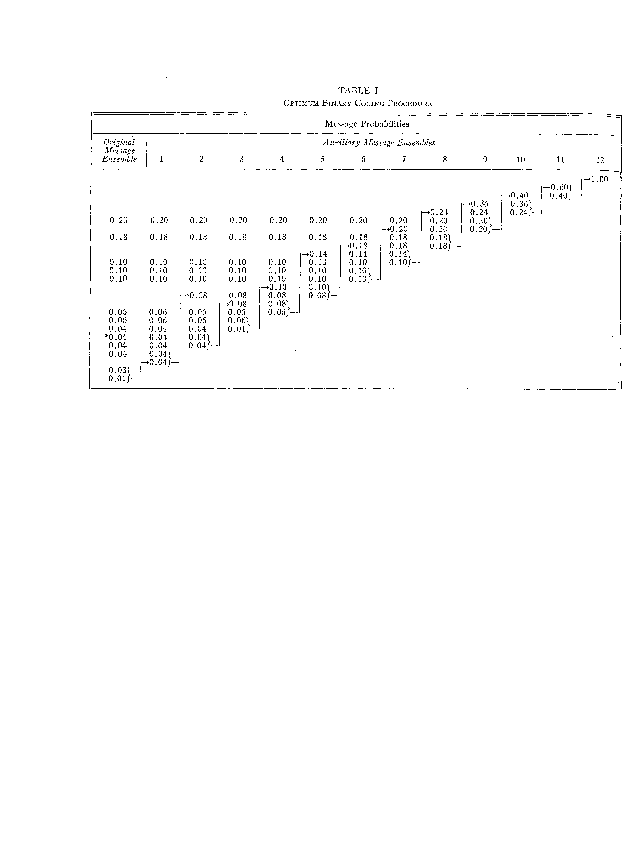
\includegraphics[scale=1.35]{img/C3_figure_1}
    \caption{Huffman Coding Diagram \cite{Huffman_1952}}
\end{figure}


\paragraph{Applications} JPEG, MP3, MPEG, PKZIP.

\begin{theorem}[Huffman Code Theorem]
    \mbox{}\\
    For the given source $S$, the Huffman algorithm produces a minimum average length UD-code which is an instantaneous code.
\end{theorem}

\begin{proposition}[Knuth]
    \mbox{}\\
    For a Huffman code created by the given algorithm, the average code word length is sum of all the probabilities at child nodes.
\end{proposition}

\subsubsection{Properties of Huffman Codes}

\begin{enumerate}
    \item The place high strategy always produces a minimum variance Huffman code .
    \item If there are $2^{n}$ equally likely source symbols then the Huffman code is a block code of length $n$.
    \item If for all $j$, $3p_{j} \geq 2 \sum_{k=j+1}^{q}p_{k}$ then the Huffman code is a comma code.
    \item Small changes in the pi can change the Huffman code substantially, but have little effect on the average length $L$. This effect is smaller with smaller variance.
\end{enumerate}

\subsubsection{Radix $r$ Huffman Codes}
For $r$ radix Huffman codes, which $r \geq 3$, we have a better strategy by adding some dummy variables \cite{cmuLec8}.

For a $r$ radix encoding, the procedure is similar except $r$ least probable symbols are merged at each step. Since the total number of symbols may not be enough to allow $r$ variables to be merged at each step, we might need to add some dummy symbols with $0$ probability before constructing the Huffman tree.

How many dummy symbols need to be added? Since the first iteration merges $r$ symbols and then each iteration combines $r-1$ symbols with a merged symbols, if the procedure is to last for $k$ (some integer number of) iterations, then the total number of source symbols needed is $1+k(r-1)$. So before beginning the Huffman procedure, we add enough dummy symbols so that the total number of symbols look like $1+k(r-1)$ for the smallest possible value of $k$.

\begin{remark}
    \mbox{}
    \begin{enumerate}
        \item If more than two symbols have the same probability at any iteration, then the Huffman coding may not be unique (depending on the order in which they are merged). However, all Huffman codings on that alphabet are optimal in the sense they will yield the same expected code length.	
        \item 	One might think of another alternate procedure to assign small code lengths by building a tree top-down instead, e.g. divide the symbols into two sets with almost equal probabilities and repeating. While intuitively appealing, this procedure is suboptimal and leads to a larger expected code length than the Huffman encoding. You should try this on the symbol distribution described above.
    \end{enumerate}
\end{remark}

\subsubsection{Extensions of Huffman Coding}

\subsection{Markov Sources}

\subsubsection{Introduction}

A finite-state Markov chain is a sequence $S_{0},S_{1}, \cdots$ of discrete random sym­bols from a finite alphabet, $S$. There is a probability mass function (pmf) $q_{0}(s), s \in S$ on $S_{0}$, and there is a conditional pmf $Q(s|s^{\prime})$ such that for all $m \geq 1$, all $s \in S$, and all $s^{\prime} \in S$,
    \[{\mathrm Pr}(S_{k}=s|S_{k-1}=s^{\prime})={\mathrm Pr}(S_{k}=s|S_{k-1}=s^{\prime},\cdots,S_{0}=s_{0})=Q(s|s^{\prime})\]
    There is said to be a \emph{transition} from $s^{\prime}$ to $s$, denoted $s^{\prime} \to S$, if $Q(s|s^{\prime})>0$. \cite{mitCh2}

\subsubsection{Transition Matrix}

The matrix $M = (p_{ij})$ is called the transition matrix of the Markov process, which could be displayed as $(\mathrm{from}\ s_{j}) \rightarrow (p_{ij}) \rightarrow (\mathrm{to}\ s_{i})$.

\begin{remark}
    \mbox{}
    \begin{itemize}
        \item \quad $P(s_{1}|s{j}) + P(s_{2}|s{j}) + \cdots + P(s_{q}|s{j}) = 1$
        \item \quad $p_{1j} + p_{2j} + \cdots + p_{qj} = 1, \; \mathrm{for}\ j = 1, \cdots, q$
    \end{itemize}
\end{remark}

\[
\begin{bmatrix}
    p_{11} & p_{12} & \cdots & p_{1j} \\
    p_{21} & p_{22} & \cdots & p_{2j} \\
    \vdots & \vdots & \ddots & \vdots \\
    p_{i1} & p_{i2} & \cdots & p_{ij}
\end{bmatrix}
\]

\subsubsection{Huffman Coding for Stationary Markov Sources}

\subsection{Arithmetic Coding}

Arithmetic coding is very efficient and approaches the entropy limit faster than Huffman coding without any contradiction because the arithmetic coding is not a UD-code. The idea is to assign a subinterval of $[0, 1) \subseteq \mathbb{R}$ to the message and successively narrow this subinterval down as each symbol is encoded. The message must end with a stop symbol $\bullet$, which could be displayed as 
    \[s_{a}s_{b}s_{c}s_{d}s_{e} \cdots s_{n} \bullet,\]
    and after the subinterval corresponding to the message plus $\bullet$ is found, then any suitable \emph{single number} in the subinterval is transmitted -- this is the actual code number or codeword.

\subsubsection{Encoding}

Firstly, to each symbol is associated a subinterval of $[0, 1)$ whose length is proportional to the relative frequency of the symbol. These subintervals are chosen so they do not overlap, but fill $[0, 1)$.

If the ``message so far'' subinterval is $[s, s+w)$ where $s$ is the start, $w$ is the width and the next symbol has associated subinterval $[s^{\prime}, s^{\prime}+w^{\prime})$ then the new message subinterval is the $[s^{\prime}, s^{\prime}+w^{\prime})$ part of $[s, s+w)$.

That is, the new message subinterval becomes \[[s+s^{\prime}w, (s+s^{\prime}w)+w^{\prime}w).\]

It could be shown as a list step by step:

\begin{itemize}
    \item \textbf{Crop} $[0, 1)$ as current interval.
    \item \textbf{Partition} the current interval $[0, 1)$ into subintervals of length $p_{1} \cdots p_{q}$, which $p_{q}$ is a stop symbol $\bullet$.
    \item \textbf{Crop} the $i_{1}^{\mathrm{th}}$ subinterval as the current interval.
    \item \textbf{Partition} the current interval $[\mathrm{new\ start}, \mathrm{new\ end})$ into subintervals of length $p_{1} \cdots p_{q}$, which $p_{q}$ is a stop symbol $\bullet$.
    \item \textbf{Crop} the $i_{2}^{\mathrm{th}}$ subinterval as the current interval, which is also a sub-subinterval of the initial interval $[0, 1)$.
    \item \textbf{Repeat} this process until the whole message has been encoded.
\end{itemize}

\begin{figure}[htbp]
    \center
    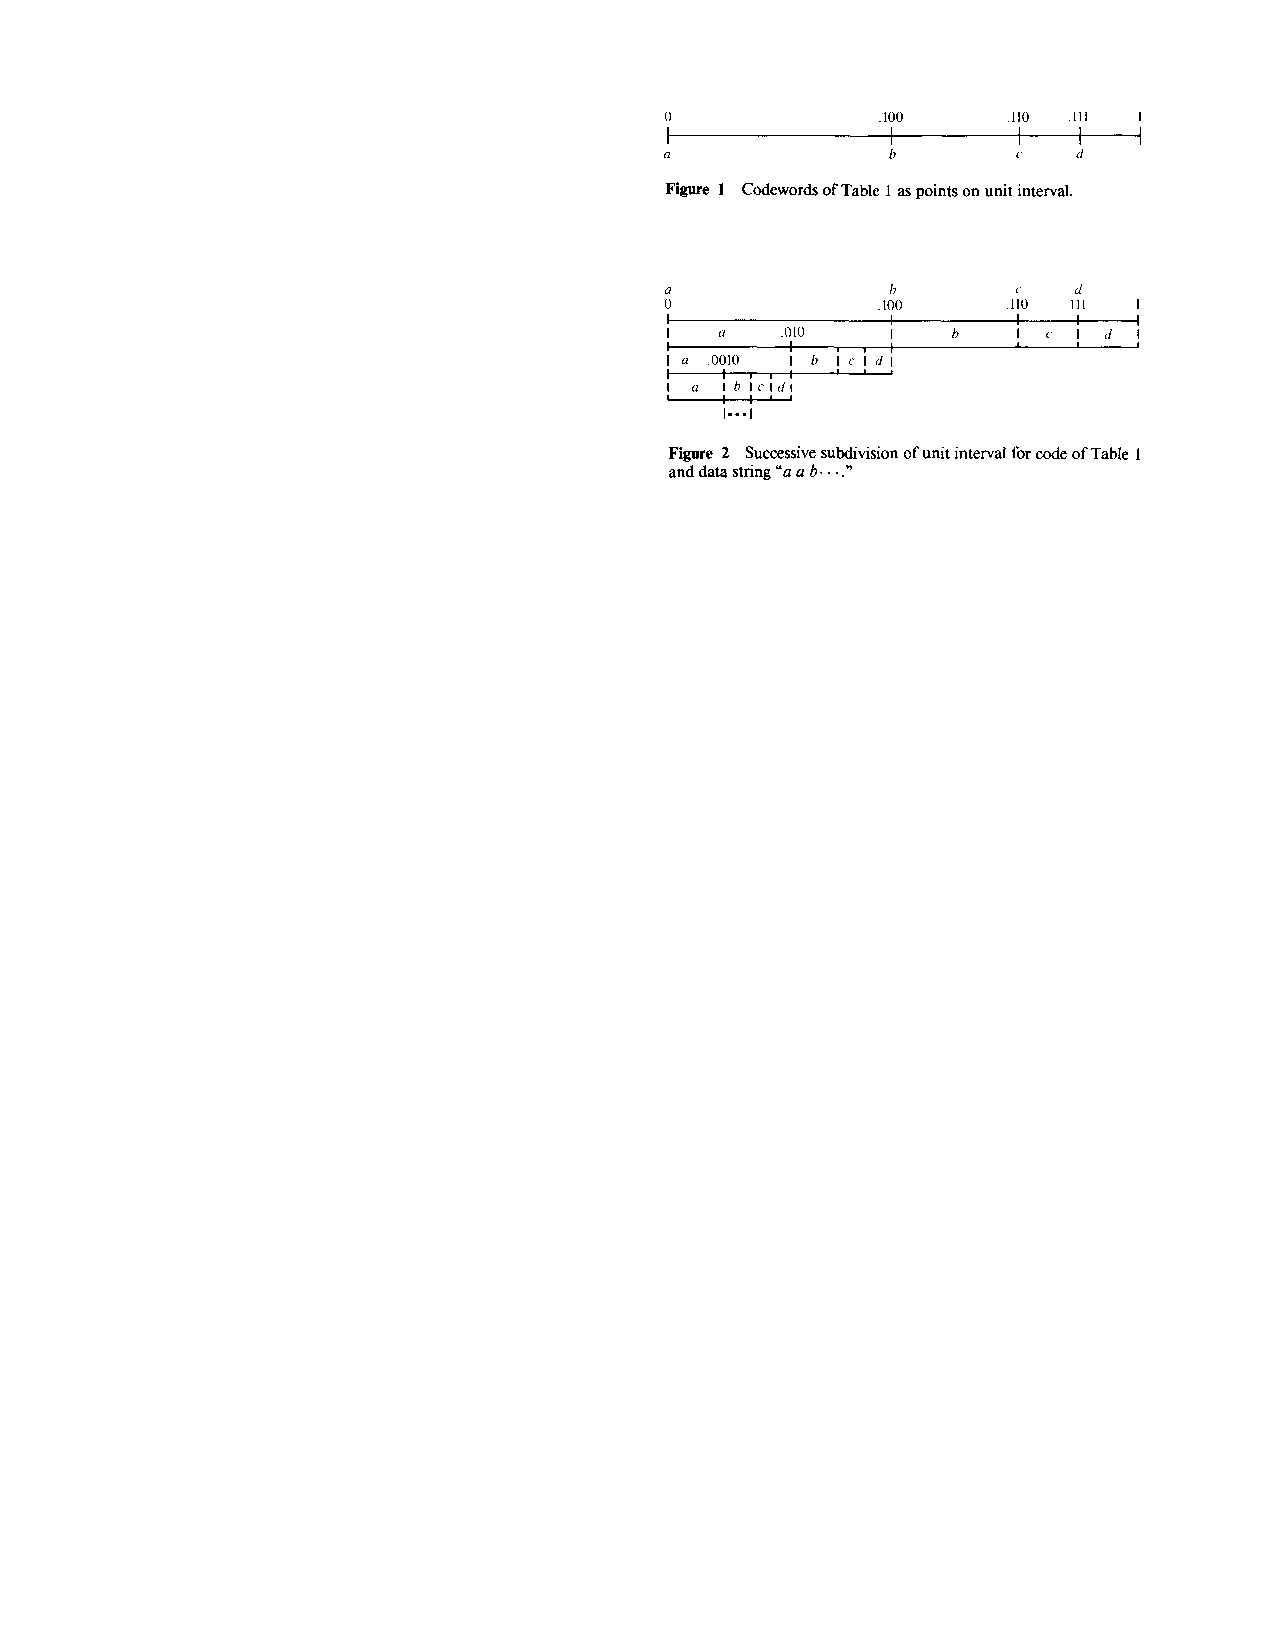
\includegraphics[scale=1.35]{img/C3_figure_2}
    \caption{Arithmetic Coding Diagram \cite{Langdon_1984}}
\end{figure}

\subsubsection{Decoding}

We reverse the above, by finding which of the symbol subintervals contains
the code number. This then gives the first symbol of the message.

The code number is then re-scaled to that interval as follows.
If $x$ is the code number and it lies in the subinterval $[s, s+w)$,
then the rescaled code number is $\dfrac{x-s}{w}$. The process is repeated until
the stop symbol $\bullet$ is encountered.

\begin{remark}
    \mbox{}
    \begin{enumerate}
        \item Without the stop symbol, decoding would usually go on forever.
        \item It is possible to implement arithmetic coding and decoding using integer arithmetic, and if we use binary representation for the subintervals then it can actually be done using binary arithmetic.  Successive digits can be transmitted as soon as they are finalized; that is, when both start and end points of the interval agree to sufficiently many significant places.  Decoding can also be done as the digits arrive.  Hence arithmetic coding does not need much memory.
        \item We have described a static version of arithmetic coding.  But the process can also be made adaptive by continually adjusting the start/width values for symbols while decoding takes place.
    \end{enumerate}    
\end{remark}

\subsection{Dictionary Methods}

\paragraph{Examples} \textbf{Ziv, LZ77, LZ78 and LZW} are four dictionary compressing methods.
Dictionary-based algorithms do not encode single symbols as variable-length bit strings; they encode variable-length strings of symbols as single tokens:

\begin{itemize}
    \item The tokens form an index into a phrase dictionary.
    \item If the tokens are smaller than the phrases they replace, compression occurs.
\end{itemize}

Consider the Random House Dictionary of the English Language, Second edition, Unabridged. Using this dictionary, the string
    \[\text{A good example of how dictionary based compression works}\]
can be coded as
    \[1/1 \quad 822/3 \quad 674/4 \quad 1343/60 \quad 928/75 \quad 550/32 \quad 173/46 \quad 421/2\]

\paragraph{Coding} Uses the dictionary as a simple lookup table.

\begin{itemize}
    \item Each word is coded as x/y, where, x gives the page in the dictionary and y gives the number of the word on that page.
    \item The dictionary has 2,200 pages with less than 256 entries per page: Therefore x requires 12 bits and y requires 8 bits, i.e., 20 bits per word (2.5 bytes per word).
    \item Using ASCII coding the above string requires 48 bytes, whereas our encoding requires only $20\ (2.5 \times 8)$ bytes: 50\% compression. \cite{utexasMbs}
\end{itemize}

\paragraph{Applications} GZIP, GIF, POSTSCRIPT.

\subsubsection{Encoding}

Start with an empty dictionary and set $r = m$. (Here $r$ is the part of the message which we have not yet encoded.) Let “$+$” denote concatenation of symbols. Repeat the following steps until $r$ is empty:
\begin{enumerate}
    \item Let s be the longest prefix of $r$ which corresponds to a dictionary entry. If there is no such prefix then set $s = \emptyset$. (By prefix we mean a subsequence of $r$ which begins at the first symbol.)
    \item Suppose that $s$ is in line $l$ of the dictionary, and put $l = 0$ if $s = \emptyset$. Add a new dictionary entry for $s + c$, where $c$ is the next symbol after $s$ in $r$. Output $(l, c)$ to the encoding and delete $s + c$ from $r$.
\end{enumerate}

\subsubsection{Decoding}

\begin{enumerate}
    \item Start with an empty dictionary.
    \item If the next code pair is $(l, c)$ then output $D(l) + c$ to the message, where $D(l)$ denotes entry $l$ of the dictionary and $D(0) = \emptyset$.
    \item Also add $D(l) + c$ to the dictionary. Repeat until all code pairs have been processed.
    \item The dictionary after the decoding process is exactly the same as the dictionary after the encoding process.
\end{enumerate}

\newpage

\setcounter{section}{6}

\section{Cryptography (Ciphers)}

\subsection{Introduction}

A \textbf{message} m from among a set $M$ of all possible messages is \textbf{encrypted} (or enciphered or encoded), using one of a set $\{E_{k}\}$ of \textbf{encryption functions} (or cryptographic transformations)
    \[E_{k}: M \rightarrow C\]
    into an \textbf{encrypted message} $c \in C$, where $C$ is the set of all possible encrypted messages.

The encryption function $E_{k}$ depends on the particular \textbf{key} $k$ chosen from a set $K$ of all possible keys.

The encrypted message $c$ is then transmitted to the receiver, who decrypts it using the decryption function
    \[D_{k}: C \rightarrow M\]
    using the same key $k$. Here Dk is the inverse of $E_{k}$, which means that
    \[D_{k}(c)=D_{k}(E_{k}(m))=m\]
We also call $m$ the \textbf{plaintext} and $c$ the \textbf{cipher text}.

\begin{figure}[htbp]
    \center
    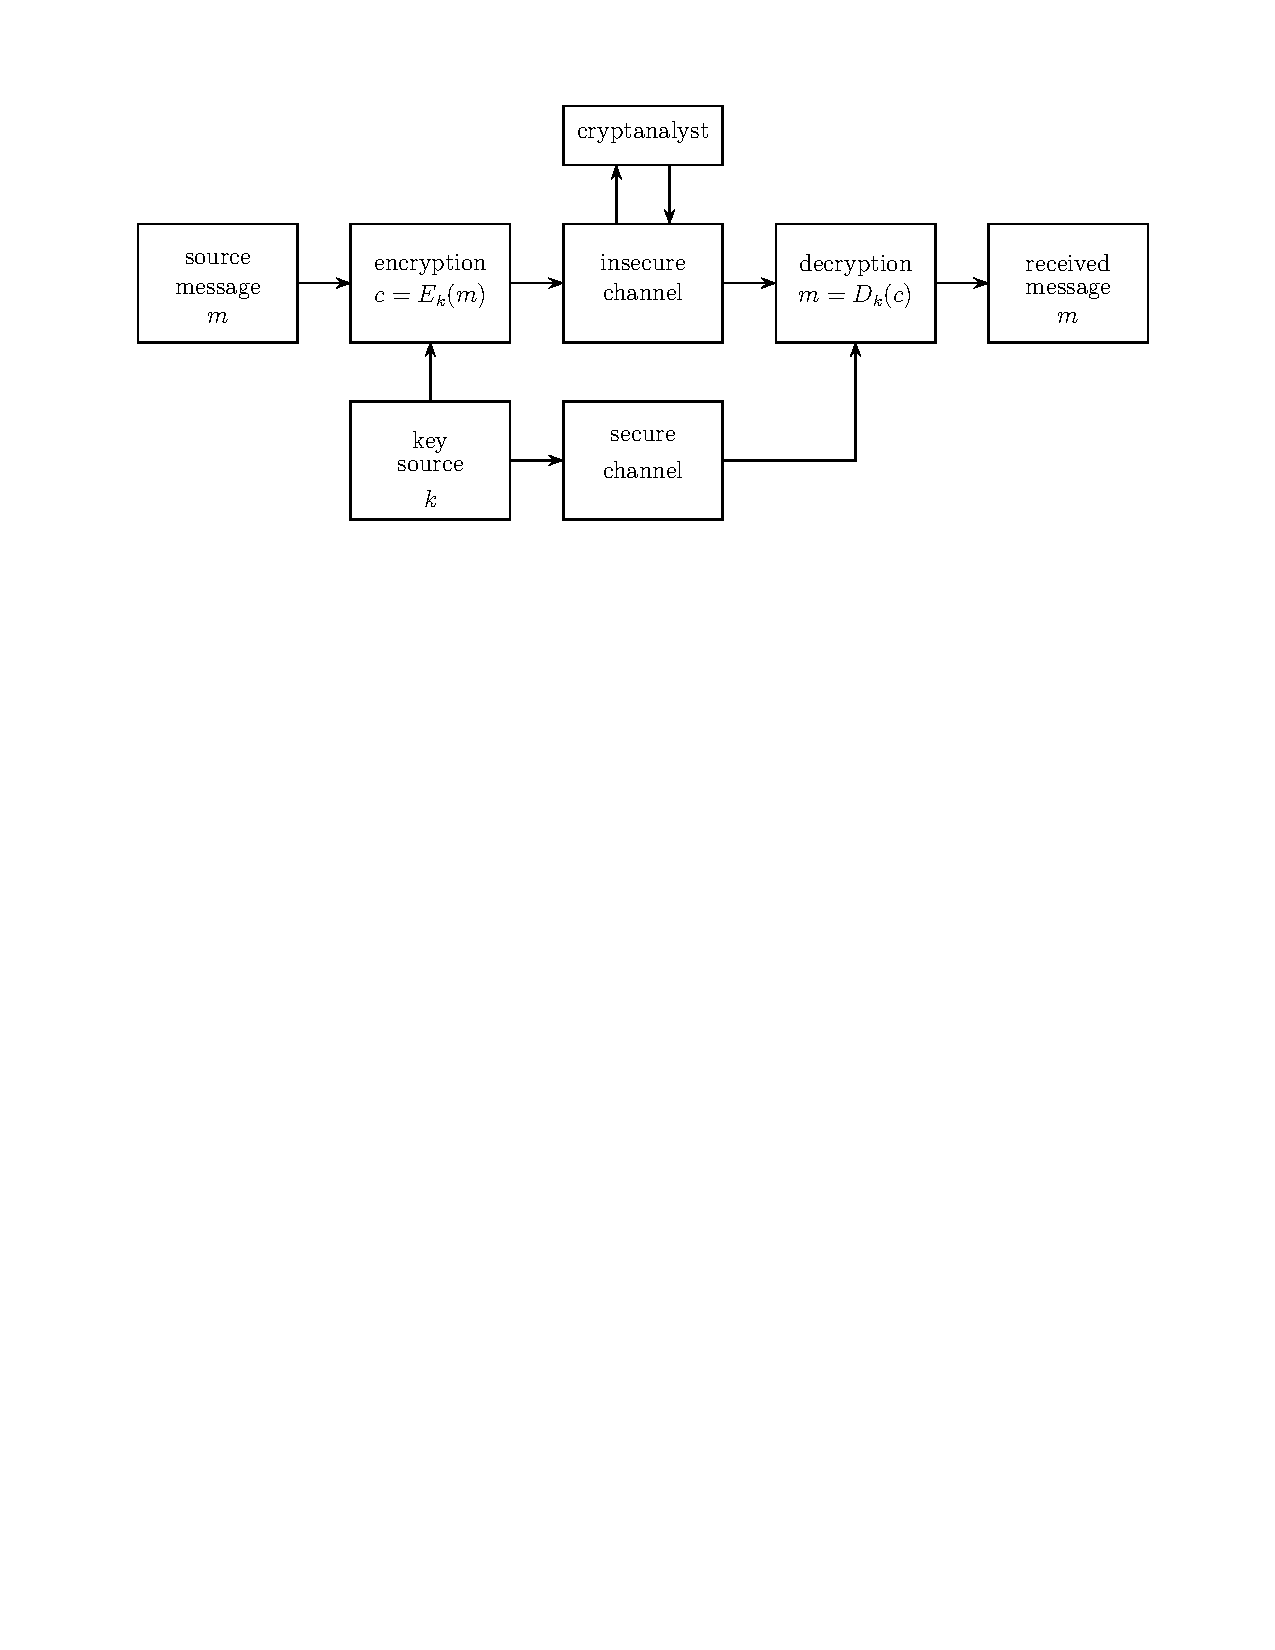
\includegraphics[width=\textwidth]{img/C7_figure_1}
    \caption{Cryptography}
\end{figure}

\begin{principle}[Kerckhoffs's Principle of Cryptography \cite{Kerckhoffs_1883}]
    \mbox{}\\
    \begin{enumerate}
        \item The system must be practically, if not mathematically, indecipherable;
        \item It should not require secrecy, and it should not be a problem if it falls into enemy hands;
        \item It must be possible to communicate and remember the key without using written notes, and correspondents must be able to change or modify it at will;
        \item It must be applicable to telegraph communications;
        \item It must be portable, and should not require several persons to handle or operate;
        \item Lastly, given the circumstances in which it is to be used, the system must be easy to use and should not be stressful to use or require its users to know and comply with a long list of rules.
    \end{enumerate}
\end{principle}

Claude Shannon reformulated this principle as "one ought to design systems under the assumption that the enemy will immediately gain full familiarity with them", which called

\paragraph{Shannon's Maxim} "The enemy knows the system."

\subsection{Some Classical Cryptosystems}

\subsubsection{Caesar Cipher}

Cyclically shift each letter $k$ places forward, e.g. for $k = 3$, which is also used by Roman dictator Gaius Julius Caesar himself.

\begin{center}
    \texttt{
         plain \quad A B C D E F G H I J K L M N O P Q R S T U V W X Y Z\\
        cipher \quad D E F G H I J K L M N O P Q R S T U V W X Y Z A B C
    }
\end{center}

If letters are represented by $\mathbb{Z}_{26}$, then we have, for key $k$,

\begin{align*}
    E_{k}(i) &= i+k \pmod{26} \text{\quad for all } i\\
    \text{and \quad} D_{k}(j) &= j-k \pmod{26} \text{\quad for all } j.\\
\end{align*}

There are only 26 keys $k$, so this cipher is easily broken by simply trying all possible keys until it makes sense.

\subsubsection{Monoalphabetic Substitution Cipher}

Replace each letter by another character, such as

\begin{center}
    \texttt{
         plain \quad A B C D E F G H I J K L M N O P Q R S T U V W X Y Z\\
        cipher \quad P Q S T U V W X Y Z C O D E B R A K I N G F H J L M
    }
\end{center}

The keyword \texttt{"CODEBREAKING"} starting at \texttt{K} leads to a more memorable permutation, but the code would be easier to break.

Let $\pi$ be the permutation of $\mathbb{Z}_{26}$ used, then

\begin{align*}
    E_{k}(i) &= \pi(i) \text{\quad\quad \,for all } i\\
    \text{and \quad} D_{k}(j) &= \pi^{-1}(j) \text{\quad for all } j.\\
\end{align*}

If we only use alphabetical characters as key $k$, there are still $26! \approx 4 \times 10^{26}$ possible keys so it is impossible to try them all.

\subsubsection{Transposition Cipher}

Mix up the order of the letters by dividing them up into blocks of length $l$ and applying a permutation $\pi \in \mathrm{Sym}(l)$ to the letter order. For example, with blocks of length $5$ we could use the permutation
    \[\pi = 
    \begin{pmatrix}
        1 &2 &3 &4 &5\\
        3 &1 &4 &5 &2
    \end{pmatrix}
    \quad
    \text{map 1st letter} \to \text{3rd letter, 2nd} \to \text{1st, and so on.}
    \]

The $\text{Sym}(r)$ means the symmetric group. \cite{wiki:sym}

\begin{center}
    \texttt{
         plain \quad T H I S I \; S A N E X \; A M P L E\\
        cipher \quad H I T I S \; A X S N E \;  M E A P L
    }
\end{center}

Frequency counts of pairs or triples and common sense allow these ciphers to be easily broken.

\subsubsection{Combined Systems}

\newpage

\bibliographystyle{IEEEtran}
\bibliography{References.bib}

\end{document}
